\documentclass[../report.tex]{subfiles}

\begin{document}
\par Dans une dernière partie, on va s’attacher à étudier les corrélations entre les séries temporelles de température à Bordeaux et à Ploumanac’h. 

\begin{figure}[H]
  \centering
    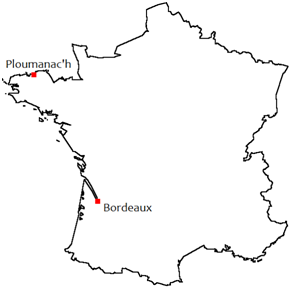
\includegraphics[width=0.7\textwidth]{images/part_3/france.png}
\end{figure}

\subsection{Étude de la \emph{cross-correlation}}

\par Le tracé de la \emph{cross-correlation} entre les deux séries temporelles révèle une corrélation forte (coefficient de 0.88) avec un maximum atteint pour un décalage de trois jours.

\begin{figure}[H]
  \centering
    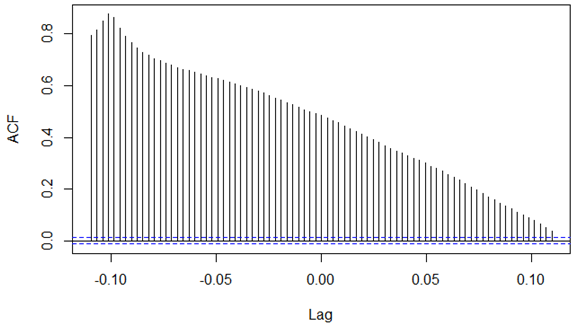
\includegraphics[width=0.7\textwidth]{images/part_3/crosscorrelation.png}
\end{figure}

\subsection{Estimation d’une copule }

\par On trace tout d’abord le graphe des températures obtenues à Ploumanac’h en fonction des températures relevées à Bordeaux.

\begin{figure}[H]
  \centering
    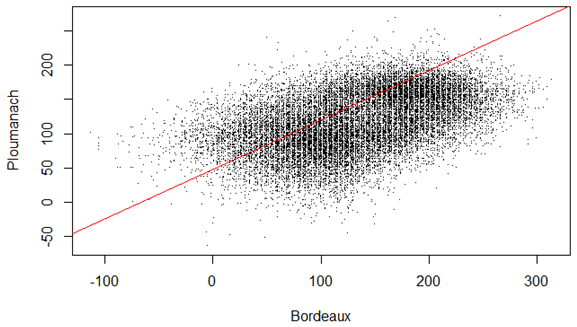
\includegraphics[width=0.7\textwidth]{images/part_3/scatterplot.png}
\end{figure}

\par La corrélation entre les deux séries est sensible et fait écho au sens physique. La corrélation de Spearman est de 0.51, celle de Kandall de 0,34, confirmant que les deux séries sont corrélées. On note à ce sujet des p-values très basses qui sont gages d’un résultat robuste : elles sont inférieures à 2e-16 dans les deux cas.

\par On peut tracer le graphe des rangs des températures à Ploumanac’h en fonction des rangs des températures à Bordeaux pour se figurer l’allure de la relation des deux séries temporelles. On ne considère ici que 2000 points par souci de lisibilité.

\begin{figure}[H]
  \centering
    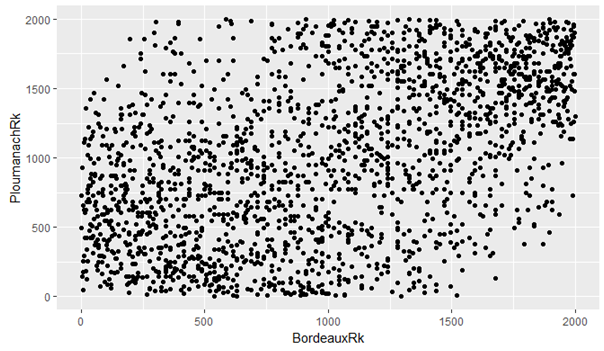
\includegraphics[width=0.7\textwidth]{images/part_3/scatterrank.png}
\end{figure}

\par Nous allons à présent choisir une copule pour modéliser la corrélation entre les deux grandeurs. On a vu que les événements extrêmes ne sont pas fortement corrélés, aussi on privilégie la copule de Clayton qui découple plus les canicules dans un premier temps.

\par On sait que pour elle en dimension 2, le tau de Kandall vaut theta/(theta+2). On en déduit la valeur du paramètre : ici ce sera 1,04.

\par On en déduit une copule qui modélise la corrélation des deux séries temporelles :

\begin{displaymath}
\bar{F} C_{\theta}^{C_l} (U_1,U_2)= \left(U_1^(-\theta)+U_2^(-\theta)-1 \right)^(\frac{1}{\theta})
\end{displaymath}

\begin{figure}[H]
  \centering
    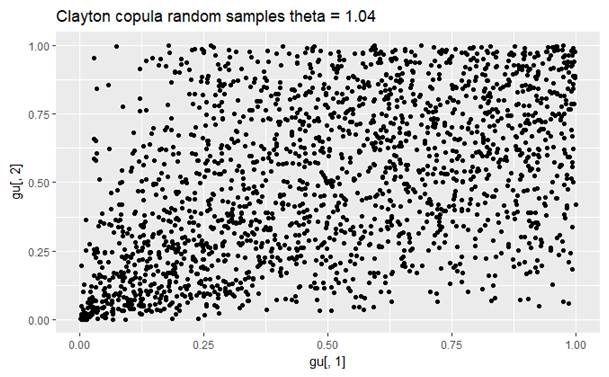
\includegraphics[width=0.7\textwidth]{images/part_3/scatterclayton.png}
\end{figure}

\par Dans un second temps, on aborde la copule de Gumbel. On sait que pour elle en dimension 2, le tau de Kandall vaut 1 – 1/theta. On en déduit la valeur de theta dans notre cas : on obtient une valeur de 1,52.

\par On en déduit une copule qui modélise la corrélation des deux séries temporelles :

\begin{displaymath}
\bar{F} C_{\theta}^{G_u} (U_1,U_2)= e^{-(-\log(U_1 )^{\theta}-\log(U_2 )^{\theta} )^(\frac{1}{\theta})}
\end{displaymath}

\begin{figure}[H]
  \centering
    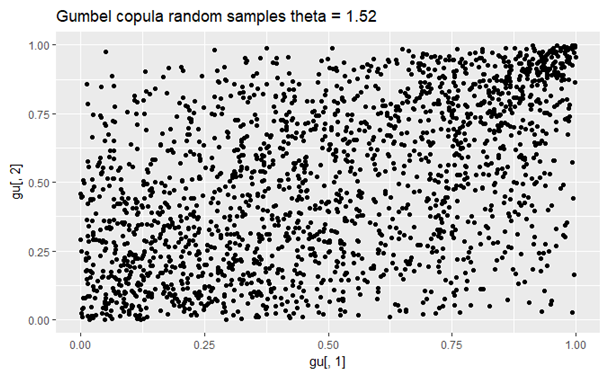
\includegraphics[width=0.7\textwidth]{images/part_3/scattergumbel.png}
\end{figure}

\par Ces tracés révèlent les limites des modélisations choisies, pour lesquelles les corrélations des événements extrêmes sont visiblement trop importantes.

\par Ainsi, on peut exhiber dans la série temporelle un trend et une saisonnalité. Néanmoins, il s'avère plus délicat de modéliser avec précision la série temporelle. Il serait nécessaire de proposer d'autres modèles, de les discuter, et de les comparer au moyen d'évaluations telles que le critère AIC.

\end{document}
